\chapter{p-p Interactions and their Simulation}
\label{chap:event:MC}


\gls{pp} interactions at the \gls{lhc} are complicated processes that span very different energy scales. 
To interpret the \gls{lhc} data it is important to both 
develop a good understanding of the physics taking place during a \gls{pp} collision and also be able to simulate 
it, to allow a comparison of the observed data with data simulated based on a specific theory, first of all the \gls{sm}.
Section \ref{sec:ppint} focuses on the description of our understanding of a \gls{pp} collision, while Section \ref{sec:eventsimul} 
discusses the event-simulation process and the main \gls{mc} generators used in the \gls{atlas} Collaboration. 



\section{p-p Interactions}
\label{sec:ppint}

In hard-scattering processes, where the momentum transfer is much higher than the proton mass \cite{Butterworth:2012fj}, 
a \gls{pp} collision is easier to understand in terms of interactions between the constituents of the protons, quarks and gluons, 
collectively referred to as partons. A schematic view of \gls{pp} event is shown in Fig. \ref{fig:sim:pp2}. In this case, the interaction of a quark and a gluon leads to a final state with a Z boson and jets. 

\begin{figure}[h]
\begin{center}
%  \subfigure[]{
%    \label{fig:Comb_syst:pt}
    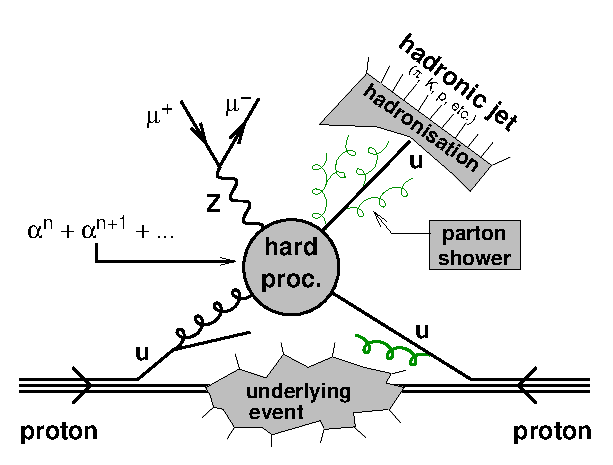
\includegraphics[width=0.58\textwidth]{figures/simul/ppcoll2}
%  }
\end{center}
 \caption{Schematic representation of a \gls{pp}, involving a quark-gluon scattering that leads to a final state consisting of a Z boson and a hard jet. Figure from Ref. \cite{Butterworth:2012fj}.}
  \label{fig:sim:pp2}
\end{figure}

As in can be understood from the figure, the hard process, which can be computed in perturbation theory, takes place between two of the proton partons; the probability that a gluon or a specific quark type takes part to the hard scattering is described the \glspl{partdf}, discussed in Section \ref{sec:ppint:hardscatter}. If the products of the hard scattering are quarks or gluons, after loosing energy by radiating other gluons (which in turn can generate quarks through gluon splitting) in the process of parton shower, they evolve into stable hadrons in the lower-energy hadronization process, which we can describe only through phenomenological models.
This picture is further complicated by the fact that also initial-state quarks and gluons can radiate. Also, the other partons not contributing to the hard scattering can interact, originating what is referred to as underlying event. 

\subsection{Factorization Theorem}
\label{sec:ppint:hardscatter}

The hard scattering between the partons inside the proton is in a kinematic regime where the \gls{qcd} coupling constant, $\alpha_s$, 
is small and therefore the partonic cross sections can be computed in perturbation theory. 
Thanks to the factorization theorem \cite{doi:10.1146}, the generic production cross section for a final state $X$ can be expressed in terms of the partonic cross section $\hat\sigma$ as:

\begin{equation}
  \label{eq:general-cross-section}
  \sigma(pp\rightarrow X) = \sum_{i,j} \int dx_1 dx_2\, 
     f_{i}(x_1,\mu_F^2)\, f_{j}(x_2,\mu_F^2)\, 
     \hat\sigma_{ij\rightarrow X}(x_1 x_2 s, \mu_R^2, \mu_F^2) \; .
\end{equation}
The $i$ and $j$ indexes run on all the possible partons, and $f_{i}(x_1,\mu_F^2)$ is the \gls{partdf} for the $i$-th parton, representing 
the distribution of probability for that parton to carry a fraction $x_1$ of the proton momentum when the proton is probed at a scale $\mu_F$
(factorization scale). $\hat\sigma_{ij\rightarrow X}$ is the partonic cross section, computer at the partonic center of mass energy \cmpart;   
it has to be noted that \cmpart is lower than the total center of mass energy, as its square is the product of square of the center of mass energy times
the fraction of the proton momentum that is carried by each of the two partons, $x_1$ and $x_2$. 
While, when considered at all orders in perturbative \gls{qcd}, the partonic cross section does not depend on $\mu_F$,
this dependence appears at any fixed order. $\hat\sigma$ depends also on the renormalization scale, $\mu_R$, which is the scale used for the evaluation of $\alpha_s$.



% factorization theorem 


%\begin{figure}[h]
%\begin{center}
%  \subfigure[]{
%    \label{fig:Comb_syst:pt}
%    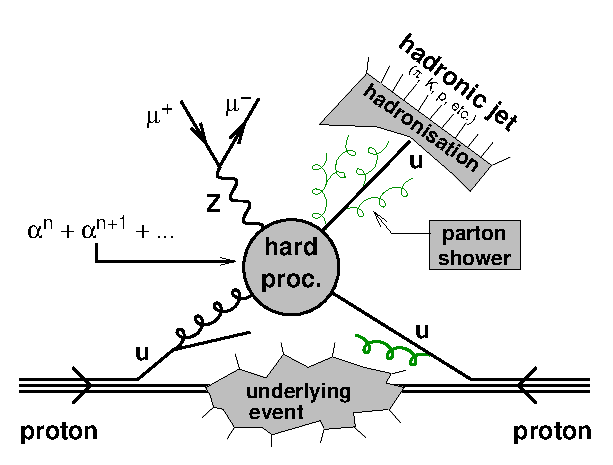
\includegraphics[width=0.48\textwidth]{figures/simul/ppcoll2}
%  }
%    \subfigure[]{
%    \label{fig:Comb_syst:pt}
%    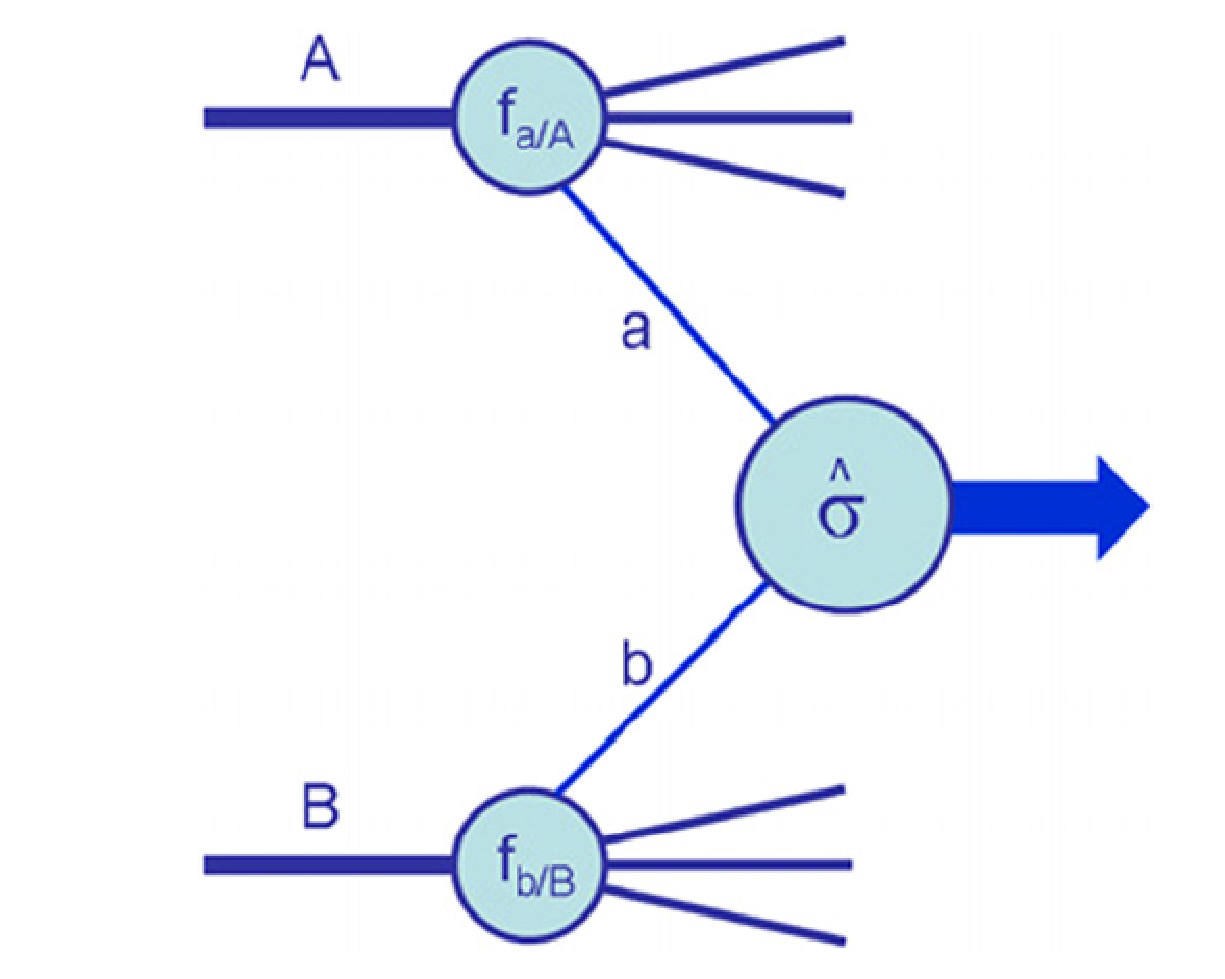
\includegraphics[width=0.48\textwidth]{figures/simul/ppcoll}
%  }
%\end{center}
% \caption{Diagrammatic structure of a generic hard-scattering process. Figure from Ref. \cite{Campbell:2006wx}.}
%  \label{fig:sim:pp}
%\end{figure}

\subsection{Parton Density Functions}

The partons inside the proton can not be observed as free particles, and therefore their \glspl{partdf} can not be computed with
perturbative \gls{qcd}. In particular, for a given scale, it is not possible to predict theoretically the probability distribution 
of the momentum fraction. Instead, once the \glspl{partdf} are known for a certain scale, their energy evolution is 
determined by the equations derived independently by Dokshitzer \cite{Dokshitzer:1977sg} , Gribov and Lipatov \cite{Gribov:1972ri}, and Altarelli and Parisi \cite{ALTARELLI1977298} (DGLAP equations):

\begin{equation}
\begin{aligned}
\frac{\partial q(x,Q^2)}{\partial {\rm log}Q^2}~&=~\frac{\alpha_s}{2\pi}~\left( P_{qq} \otimes q~+~P_{qg} \otimes g \right) \, \\
\frac{\partial g(x,Q^2)}{\partial {\rm log}Q^2}~&=~\frac{\alpha_s}{2\pi}~\left( \sum_i P_{gq} \otimes (q_i+\bar{q}_i)~+~P_{gg} \otimes g \right) \; .
\label{eq:glap1}
\end{aligned}
\end{equation}

\noindent In the expressions above, $q(x,Q^2)$ and $g(x,Q^2)$ are the quark and gluon \gls{partdf} respectively, 
$P_{ij}$ describes the $i \to j$ parton splitting function
and $\otimes$ is a symbol for the convolution integral:
\begin{equation}
P \otimes f \equiv \int^1_x\frac{dy}{y}f_q(y)~P\left(\frac{x}{y}\right).
\end{equation}

As mentioned above, the $x$ dependence has to be extracted experimentally. 

\begin{figure}[h]
\begin{center}
    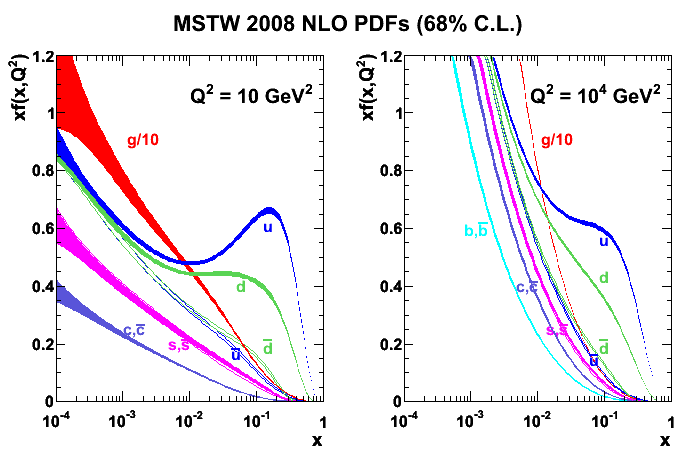
\includegraphics[width=0.8\textwidth]{figures/simul/pdf}
\end{center}
\caption{MSTW 2008 NLO PDFs at Q$^2$ = 10 GeV$^2$ and Q$^2$ = 104 GeV$^2$. Figure from Ref. \cite{Martin:2009iq}.}
 \label{fig:sim:pp}
\end{figure}


\section{Event Simulation}
\label{sec:eventsimul}

\subsection{Matrix Element}

The factorization and renormalization scales are not predetermined, and are typically set to values related to the scale of the considered physical process. 
The impact of this subjective choice is taken into account by evaluating each production cross section at different scales (typically a variation of a factor two up and down), and assigning the difference as a systematic uncertainty on the cross section estimate.

\subsection{Parton Shower}

\subsection{Matching}

\subsection{Hadronization}

\section{MC Generators}

\section{Detector Simulation}

\section{Data-driven Corrections}
